%%%%%%%%%%%%%%%%%%%%%%%%%%%%%%%%%%%%%%%%%
% Short Sectioned Assignment
% LaTeX Template
% Version 1.0 (5/5/12)
%
% This template has been downloaded from:
% http://www.LaTeXTemplates.com
%
% Original author:
% Frits Wenneker (http://www.howtotex.com)
%
% License:
% CC BY-NC-SA 3.0 (http://creativecommons.org/licenses/by-nc-sa/3.0/)
%
%%%%%%%%%%%%%%%%%%%%%%%%%%%%%%%%%%%%%%%%%

%----------------------------------------------------------------------------------------
%	PACKAGES AND OTHER DOCUMENT CONFIGURATIONS
%----------------------------------------------------------------------------------------

\documentclass[paper=a4, fontsize=11pt]{scrartcl} % A4 paper and 11pt font size
\usepackage{subcaption}
\usepackage{float}
\usepackage{listings}
\usepackage{amsmath}
\usepackage{color}

\definecolor{dkgreen}{rgb}{0,0.6,0}
\definecolor{gray}{rgb}{0.5,0.5,0.5}
\definecolor{mauve}{rgb}{0.58,0,0.82}

\lstset{frame=tb,
  language=MATLAB,
  aboveskip=3mm,
  belowskip=10mm,
  showstringspaces=false,
  columns=flexible,
  basicstyle={\small\ttfamily},
  numbers=none,
  numberstyle=\tiny\color{gray},
  keywordstyle=\color{blue},
  commentstyle=\color{dkgreen},
  stringstyle=\color{mauve},
  breaklines=true,
  breakatwhitespace=true,
  tabsize=3
}

\usepackage{CJKutf8} % chinese support
\usepackage{graphicx}

\usepackage[T1]{fontenc} % Use 8-bit encoding that has 256 glyphs
\usepackage{fourier} % Use the Adobe Utopia font for the document - comment this line to return to the LaTeX default
\usepackage[english]{babel} % English language/hyphenation
\usepackage{amsmath,amsfonts,amsthm} % Math packages

\usepackage{lipsum} % Used for inserting dummy 'Lorem ipsum' text into the template

\usepackage{sectsty} % Allows customizing section commands
\allsectionsfont{\centering \normalfont\scshape} % Make all sections centered, the default font and small caps

\usepackage{fancyhdr} % Custom headers and footers
\pagestyle{fancyplain} % Makes all pages in the document conform to the custom headers and footers
\fancyhead{} % No page header - if you want one, create it in the same way as the footers below
\fancyfoot[L]{} % Empty left footer
\fancyfoot[C]{} % Empty center footer
\fancyfoot[R]{\thepage} % Page numbering for right footer
\renewcommand{\headrulewidth}{0pt} % Remove header underlines
\renewcommand{\footrulewidth}{0pt} % Remove footer underlines
\setlength{\headheight}{13.6pt} % Customize the height of the header

\numberwithin{equation}{section} % Number equations within sections (i.e. 1.1, 1.2, 2.1, 2.2 instead of 1, 2, 3, 4)
\numberwithin{figure}{section} % Number figures within sections (i.e. 1.1, 1.2, 2.1, 2.2 instead of 1, 2, 3, 4)
\numberwithin{table}{section} % Number tables within sections (i.e. 1.1, 1.2, 2.1, 2.2 instead of 1, 2, 3, 4)

\setlength\parindent{0pt} % Removes all indentation from paragraphs - comment this line for an assignment with lots of text

%----------------------------------------------------------------------------------------
%	TITLE SECTION
%----------------------------------------------------------------------------------------

\newcommand{\horrule}[1]{\rule{\linewidth}{#1}} % Create horizontal rule command with 1 argument of height

\title{
\normalfont \normalsize 
\textsc{计算物理学15春季} \\ [25pt] % Your university, school and/or department name(s)
\horrule{0.5pt} \\[0.4cm] % Thin top horizontal rule
\huge 第五次作业解题报告 \\ % The assignment title
\horrule{2pt} \\[0.5cm] % Thick bottom horizontal rule
}

\author{霍浩岩} % Your name

\date{\normalsize\today} % Today's date or a custom date

\begin{document}
\begin{CJK*}{UTF8}{gbsn}

\maketitle % Print the title

%----------------------------------------------------------------------------------------
%	PROBLEM 1
%----------------------------------------------------------------------------------------

\section{Eigenvalue problem}
\subsection{一维无限深势阱}
写出一维无限深势阱的薛定谔方程(无量纲化之后的方程):

\begin{equation}
-\frac{\partial^2 \psi}{\partial x^2} = E \psi
\end{equation}
再加上无限深势阱带来的边界条件:
\begin{equation}
\psi(0) = \psi(1) = 0
\end{equation}
这个方程的本征函数和本征值是:
\begin{equation}
\psi_n(x) = sin(n\pi x), n=1, 2, \dots
\end{equation}
\begin{equation}
E_n = n^2\pi^2
\end{equation}

\subsection{线性代数解法}
设区间$[0, 1]$被等分成N个区间,除了两端点之外,中间有$N-1$个节点$\psi_1, \psi_2, \dots, \psi_{N-1}$。薛定谔方程变成离散化形式:

\begin{equation}
-(\frac{1}{N})^2 
\begin{bmatrix}
2 & -1 \\\\
-1 & 2 & -1 \\\\
 & \ddots & \ddots & \ddots \\\\
 & & &  -1& 2
 \end{bmatrix} 
 \begin{bmatrix}
 \psi_1 \\\\ \psi_2 \\\\ \vdots \\\\ \psi_{N-1} 
 \end{bmatrix} = \lambda 
 \begin{bmatrix}
 \psi_1 \\\\ \psi_2 \\\\ \vdots \\\\ \psi_{N-1} 
 \end{bmatrix}
\end{equation}
或者可以说,其实就是求解矩阵
\begin{equation}
\mathbf{A} = -(\frac{1}{N})^2 
\begin{bmatrix}
2 & -1 \\\\
-1 & 2 & -1 \\\\
 & \ddots & \ddots & \ddots \\\\
 & & &  -1& 2
 \end{bmatrix} 
\end{equation}
的本征值和本征向量。

\subsection{程序求解}
使用MATLAB编写程序求解本征问题:
\lstset{language=MATLAB}
\begin{lstlisting}
N = 5;
                    % for eigen problems, sparse matrix does not help!
A = full(spdiags(repmat([-1 2 -1], N-1, 1), [1 0 -1], N-1, N-1));
[Q, L] = eig(A);
\end{lstlisting}
此时,Q的所有列向量代表了归一化的本征函数,而L的对角元素乘$(-N^2)$就是对应的本征值。

\subsection{和解析解的比较}
在$N=5$时,矩阵求出的本征值为:
\begin{equation}
\lambda = 9.5492, 34.5492, 65.4508, 90.4508
\end{equation}
而真实的本征值前四个为:
\begin{equation}
\lambda = 9.8696, 39.4784, 88.8264, 157.9137
\end{equation}

再将本征矢画出来:

\begin{figure}[H]
\centering
\begin{subfigure}{70mm}
  \centering
  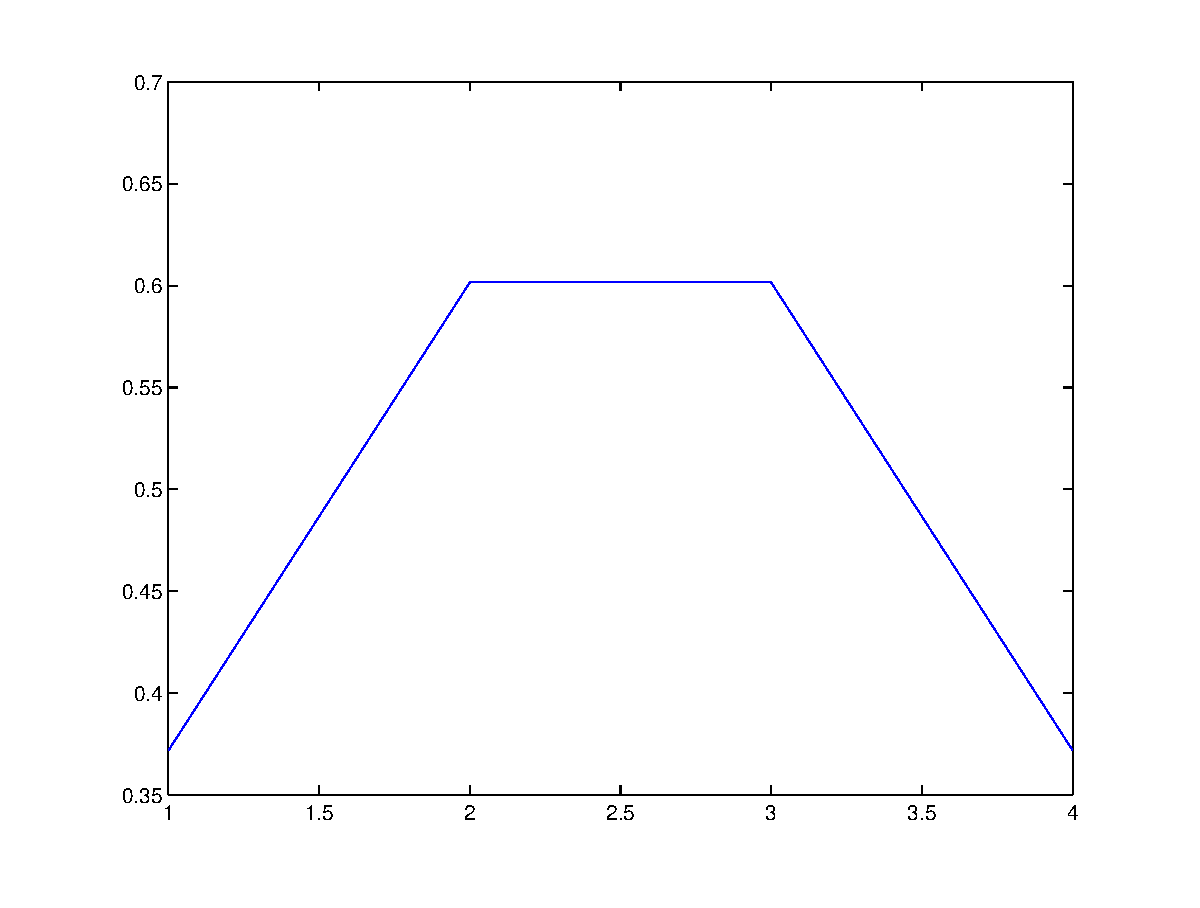
\includegraphics[width=65mm]{figure-1-1-1.eps}
  \label{fig:sub1}
\end{subfigure}
\begin{subfigure}{70mm}
  \centering
  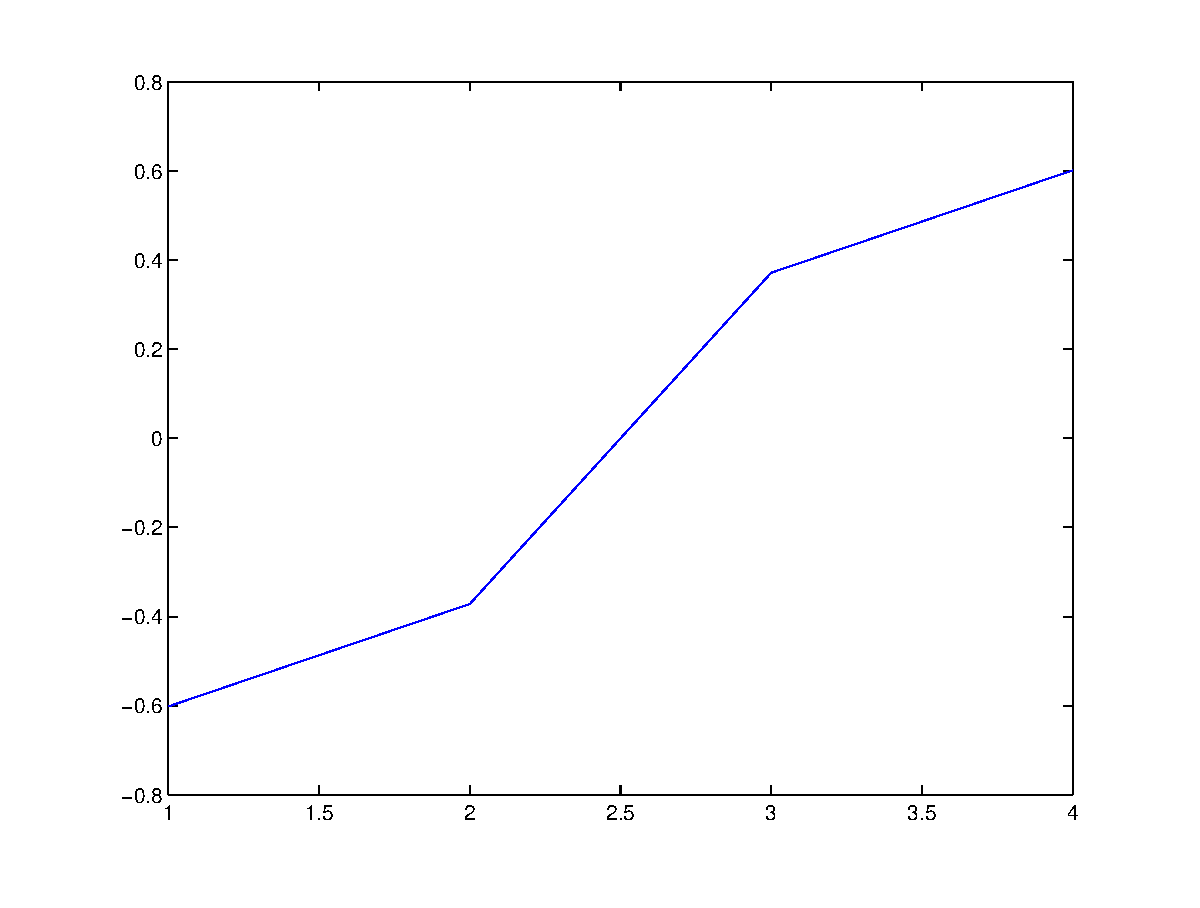
\includegraphics[width=65mm]{figure-1-1-2.eps}
  \label{fig:sub2}
\end{subfigure}
\begin{subfigure}{70mm}
  \centering
  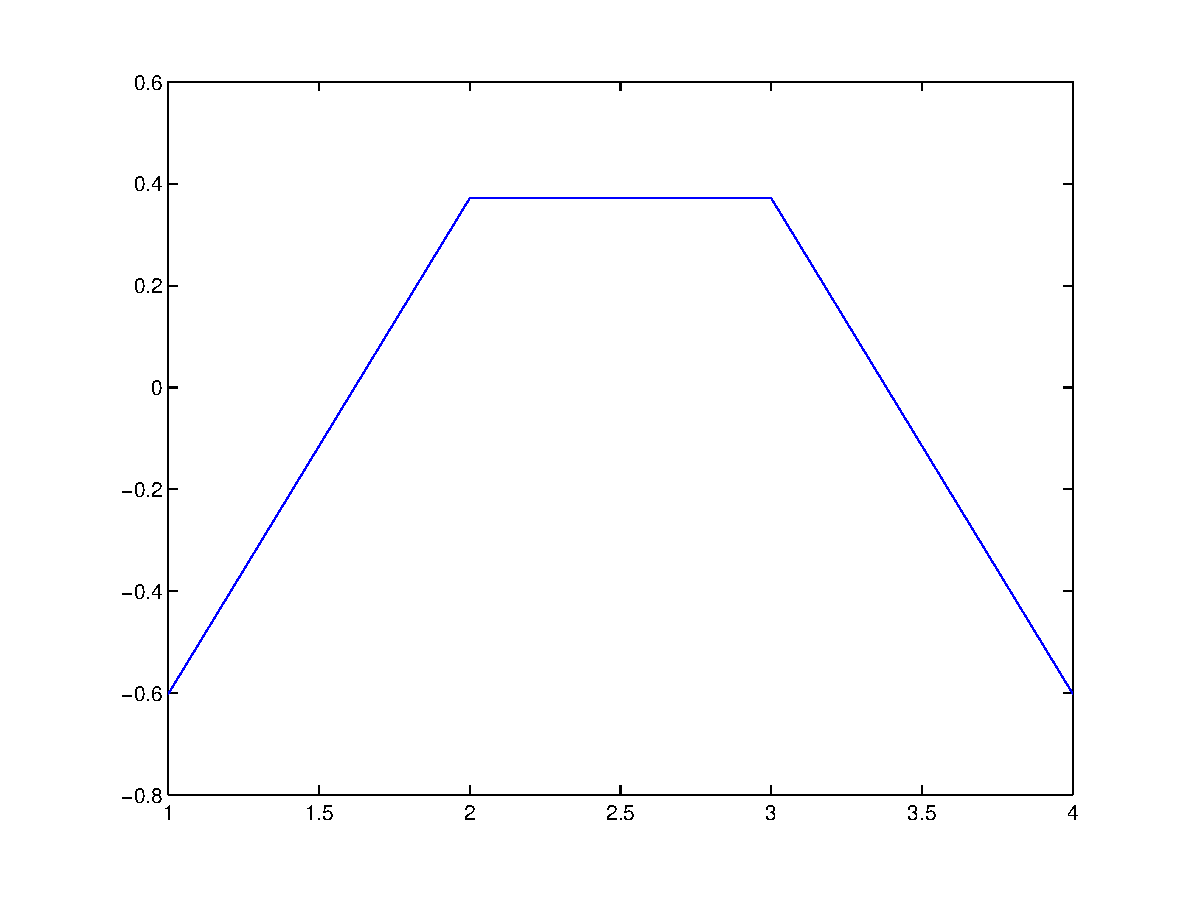
\includegraphics[width=65mm]{figure-1-1-3.eps}
  \label{fig:sub1}
\end{subfigure}
\begin{subfigure}{70mm}
  \centering
  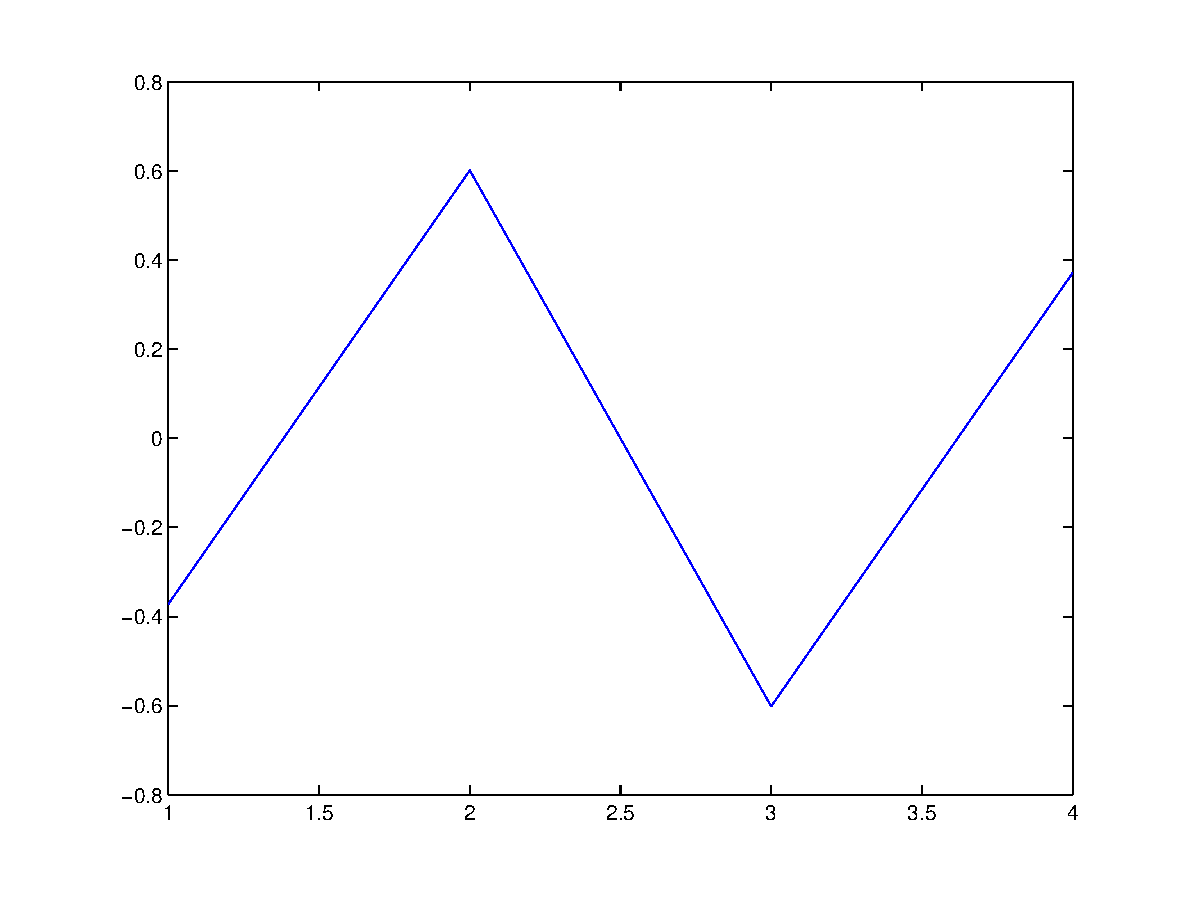
\includegraphics[width=65mm]{figure-1-1-4.eps}
  \label{fig:sub2}
\end{subfigure}
\caption{$N=5$的本征矢}
\label{fig:test}
\end{figure}
完全不正确。试着将$N$变大,例如$N=100$,然后将求出的本征值和解析本征值画在一张图里:
\begin{figure}[H]
\centering
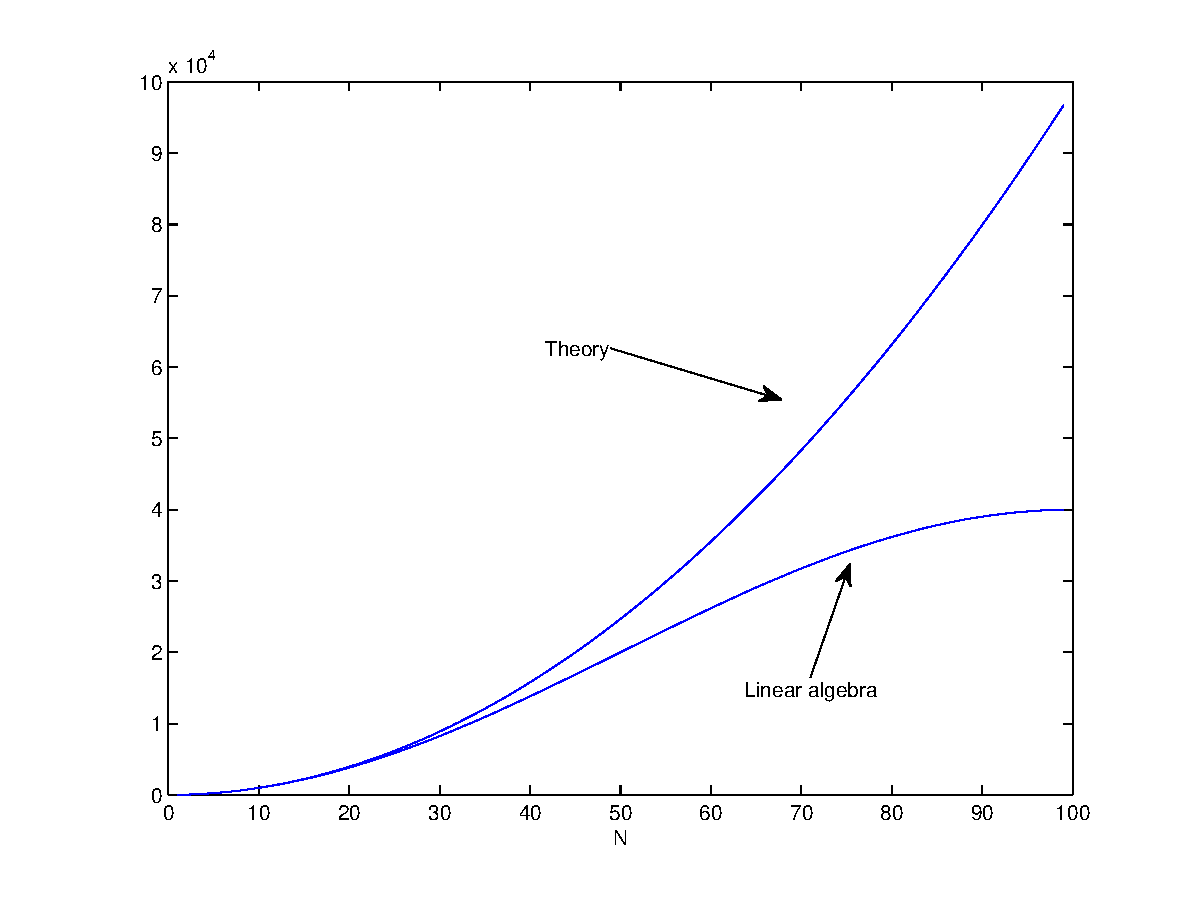
\includegraphics[width=100mm]{figure-1-2-1.eps}
\caption{$N=100$的本征值理论值和线性代数方法比较}
\label{fig:test}
\end{figure}
这个解的前面部分还是可以接受的,然而在后边的本征值却明显偏离了理论值,本来二次上升的本征值开始向下倾斜。

将$n=1, 10, 25, 50, 75, 99$的本征矢绘于图中:

\begin{figure}[H]
\centering
\begin{subfigure}{70mm}
  \centering
  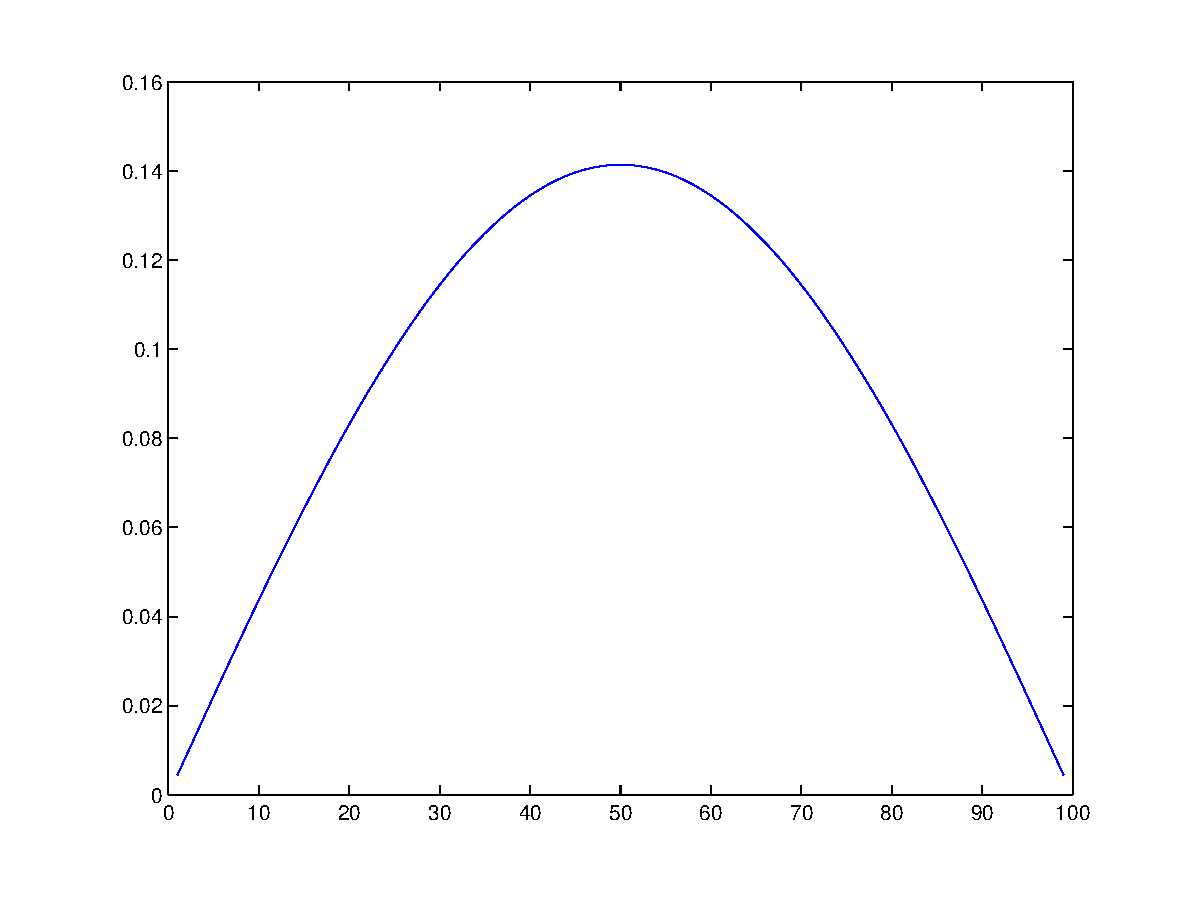
\includegraphics[width=65mm]{figure-1-2-2.eps}
  \caption{$n=1$}
  \label{fig:sub1}
\end{subfigure}
\begin{subfigure}{70mm}
  \centering
  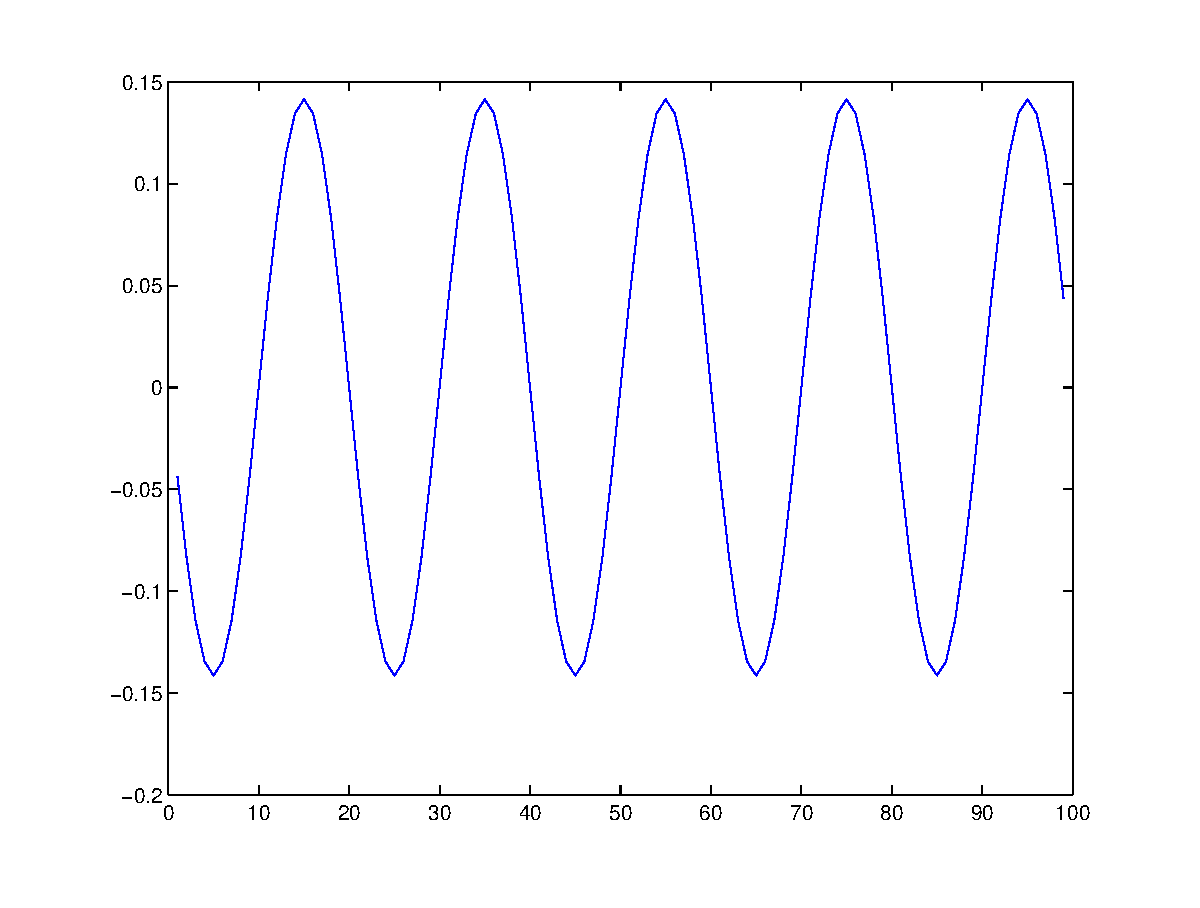
\includegraphics[width=65mm]{figure-1-2-3.eps}
  \caption{$n=10$}
  \label{fig:sub2}
\end{subfigure}
\begin{subfigure}{70mm}
  \centering
  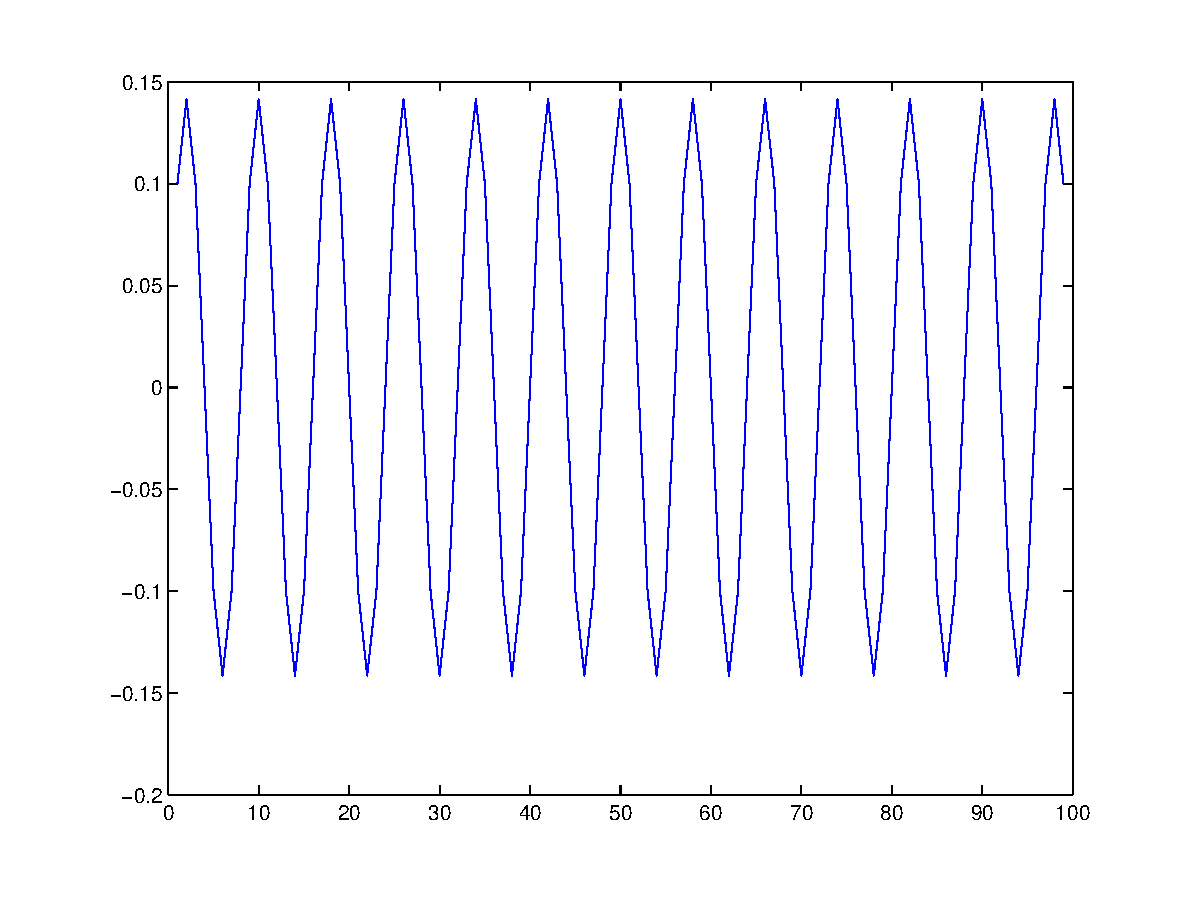
\includegraphics[width=65mm]{figure-1-2-4.eps}
  \caption{$n=25$}
  \label{fig:sub1}
\end{subfigure}
\begin{subfigure}{70mm}
  \centering
  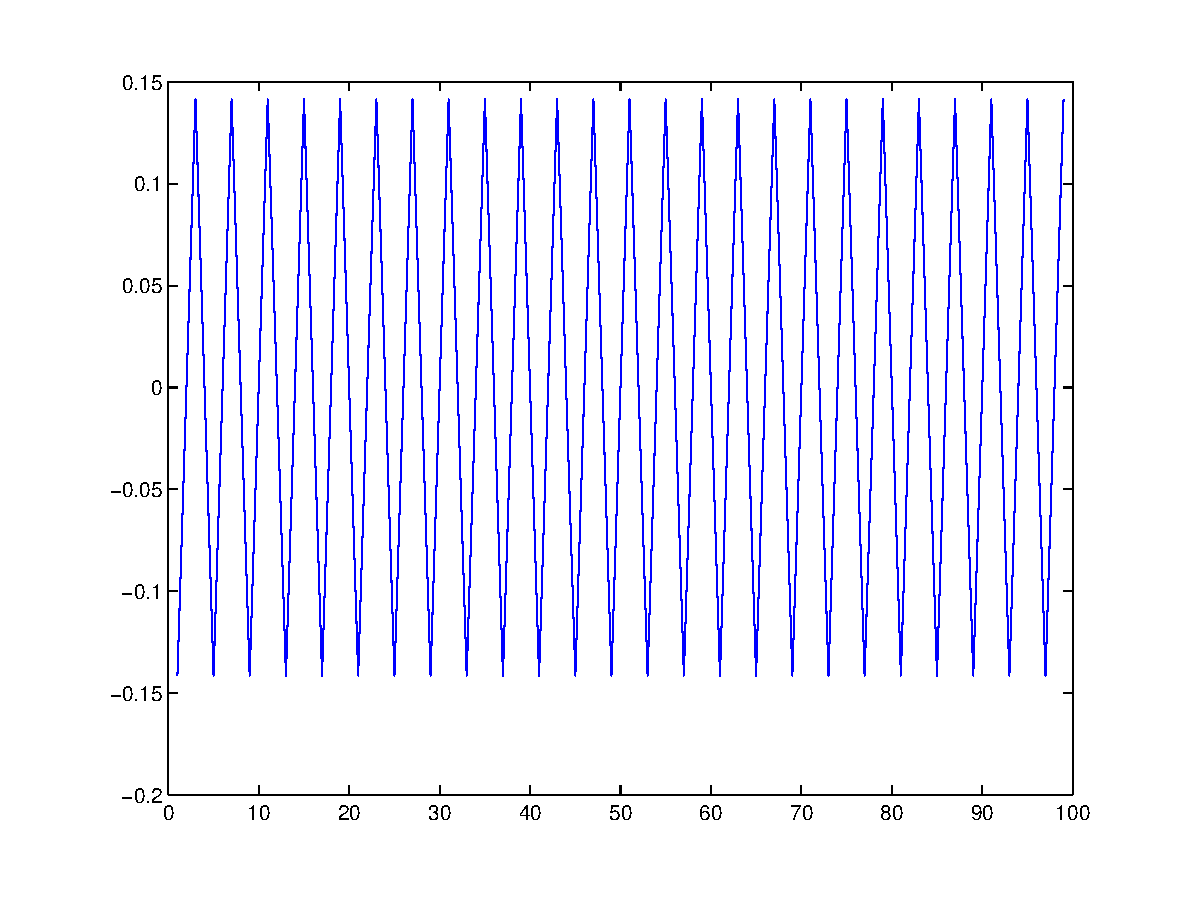
\includegraphics[width=65mm]{figure-1-2-5.eps}
  \caption{$n=50$}
  \label{fig:sub2}
\end{subfigure}
\begin{subfigure}{70mm}
  \centering
  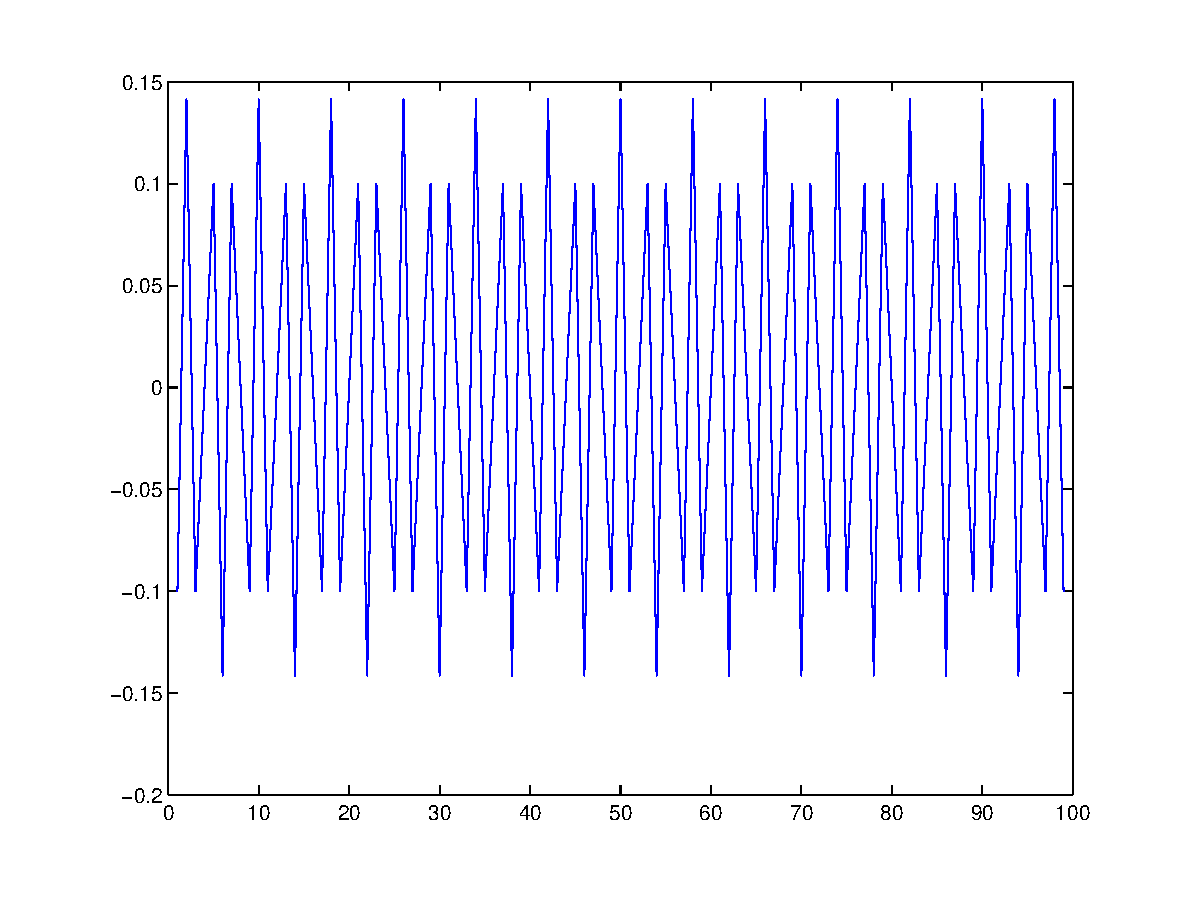
\includegraphics[width=65mm]{figure-1-2-6.eps}
  \caption{$n=75$}
  \label{fig:sub2}
\end{subfigure}
\begin{subfigure}{70mm}
  \centering
  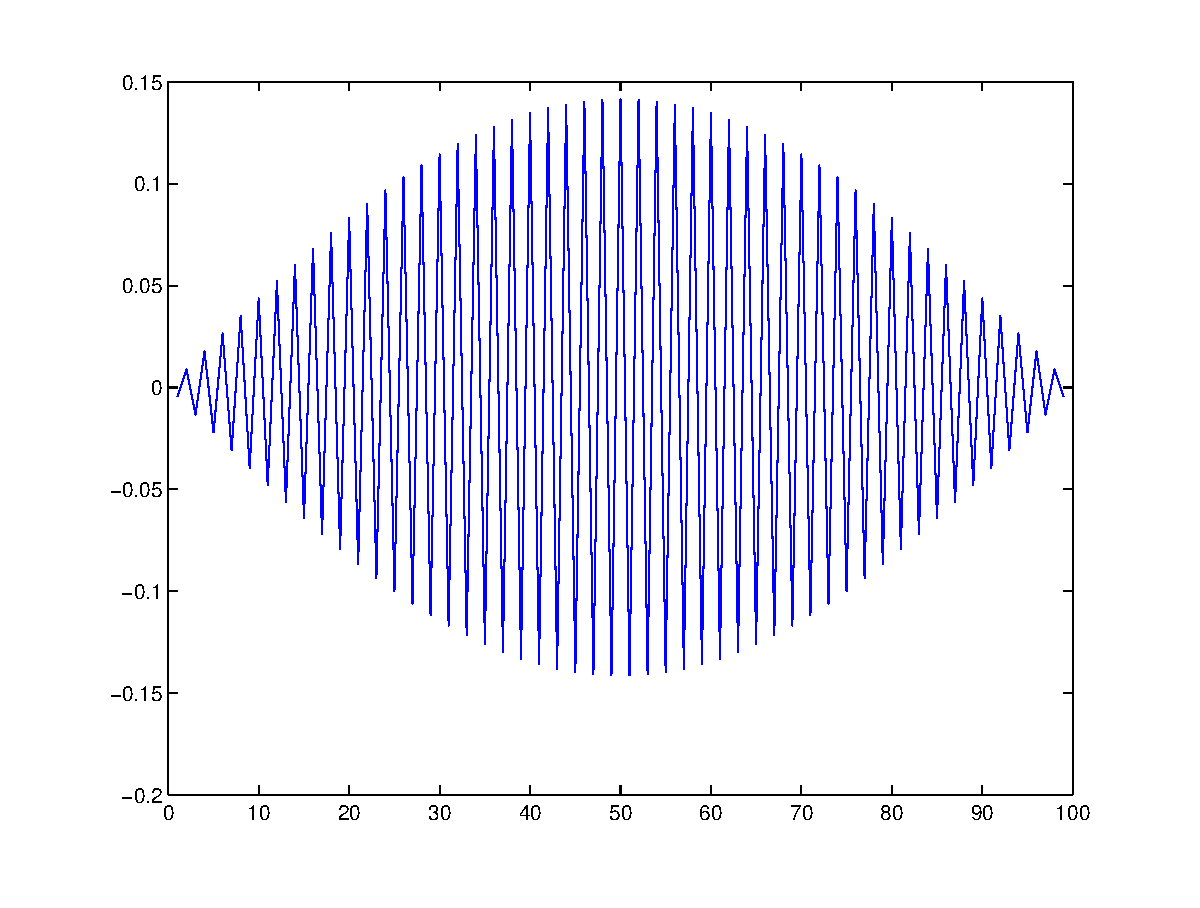
\includegraphics[width=65mm]{figure-1-2-7.eps}
  \caption{$n=99$}
  \label{fig:sub2}
\end{subfigure}
\caption{$N=100$的本征矢}
\label{fig:test}
\end{figure}
这里的问题在于,当$n$变大的时候,本征矢开始偏离解析解的$sin(n\pi x)$函数,正弦波的振幅出现“拍”的现象。对于这个问题,通过傅立叶分析可以得到一个比较形象的解释。

考虑$0 \leq x \leq 1$区间内的本征值问题,采用周期性边界条件,对方程做离散傅立叶变换,设区间被等分成$N_x$个小区间:

\begin{align}
\begin{split}
\sum_{i=1}^{N_x}e^{i\frac{2\pi}{N_x}k(i-1)}u(i) =  f(k) \\\\
\sum_{i=1}^{N_x}e^{i\frac{2\pi}{N_x}k(i-1)}u(i-1) = e^{i\frac{2\pi}{N_x}k} f(k) \\\\
\sum_{i=1}^{N_x}e^{i\frac{2\pi}{N_x}k(i-1)}u(i+1) = e^{-i\frac{2\pi}{N_x}k} f(k)
\end{split}
\end{align}
因此,$-\frac{d^2u}{dx^2}=Eu$的傅立叶变换为
\begin{equation}
4N_x^2sin^2(\frac{\pi}{N_x}k) f(k) = Ef(k)
\end{equation}

通过1.10式,我们发现本征值是一个三角函数,最大值为$4$,这和上面的结果一致。对于更高的本征值,矩阵方法有自己本身的缺陷:我们可以理解为,区间离散化后丢失了高频率的信息。所以本征值问题的矩阵解法,它的结果在本征值较大时是不可信的,要想得到较高的本征值和相应的本征基矢,就必须提高细分程度,保留更多高频率的信息。

\pagebreak
\section{Finite element method}
作业一中的问题是:
\begin{align}
\begin{split}
-\frac{\partial ^2 u}{\partial x^2} = 1, 0\le x \le 1 \\\\
u(0) = u(1) = 1
\end{split}
\end{align}
它的解析解为:
\begin{equation}
u(x) = -\frac{1}{2}x^2 + \frac{1}{2}x+1
\end{equation}
现在使用有限元算法求解,设
\begin{equation}
u(x) = v(x) + 1
\end{equation}
这样方程在边界上就都是零。选取三个hat函数:
\begin{align}
\begin{split}
\phi_1(x) = \left \{ \begin{array}{ll} 
	4x & \mbox{if } 0 \le x \le \frac{1}{4} \\
	2-4x & \mbox{if } \frac{1}{4} \le x \le \frac{1}{2}
	\end{array}
\right. \\\\
\phi_2(x) = \left \{ \begin{array}{ll} 
	-1 + 4x & \mbox{if } \frac{1}{4} \le x \le \frac{1}{2} \\
	3-4x & \mbox{if } \frac{1}{2} \le x \le \frac{3}{4}
	\end{array}
\right. \\\\
\phi_3(x) = \left \{ \begin{array}{ll} 
	-2 + 4x & \mbox{if } \frac{1}{2} \le x \le \frac{3}{4} \\
	4-4x & \mbox{if } \frac{3}{4} \le x \le 1
	\end{array}
\right.
\end{split}
\end{align}

\begin{figure}[H]
\centering
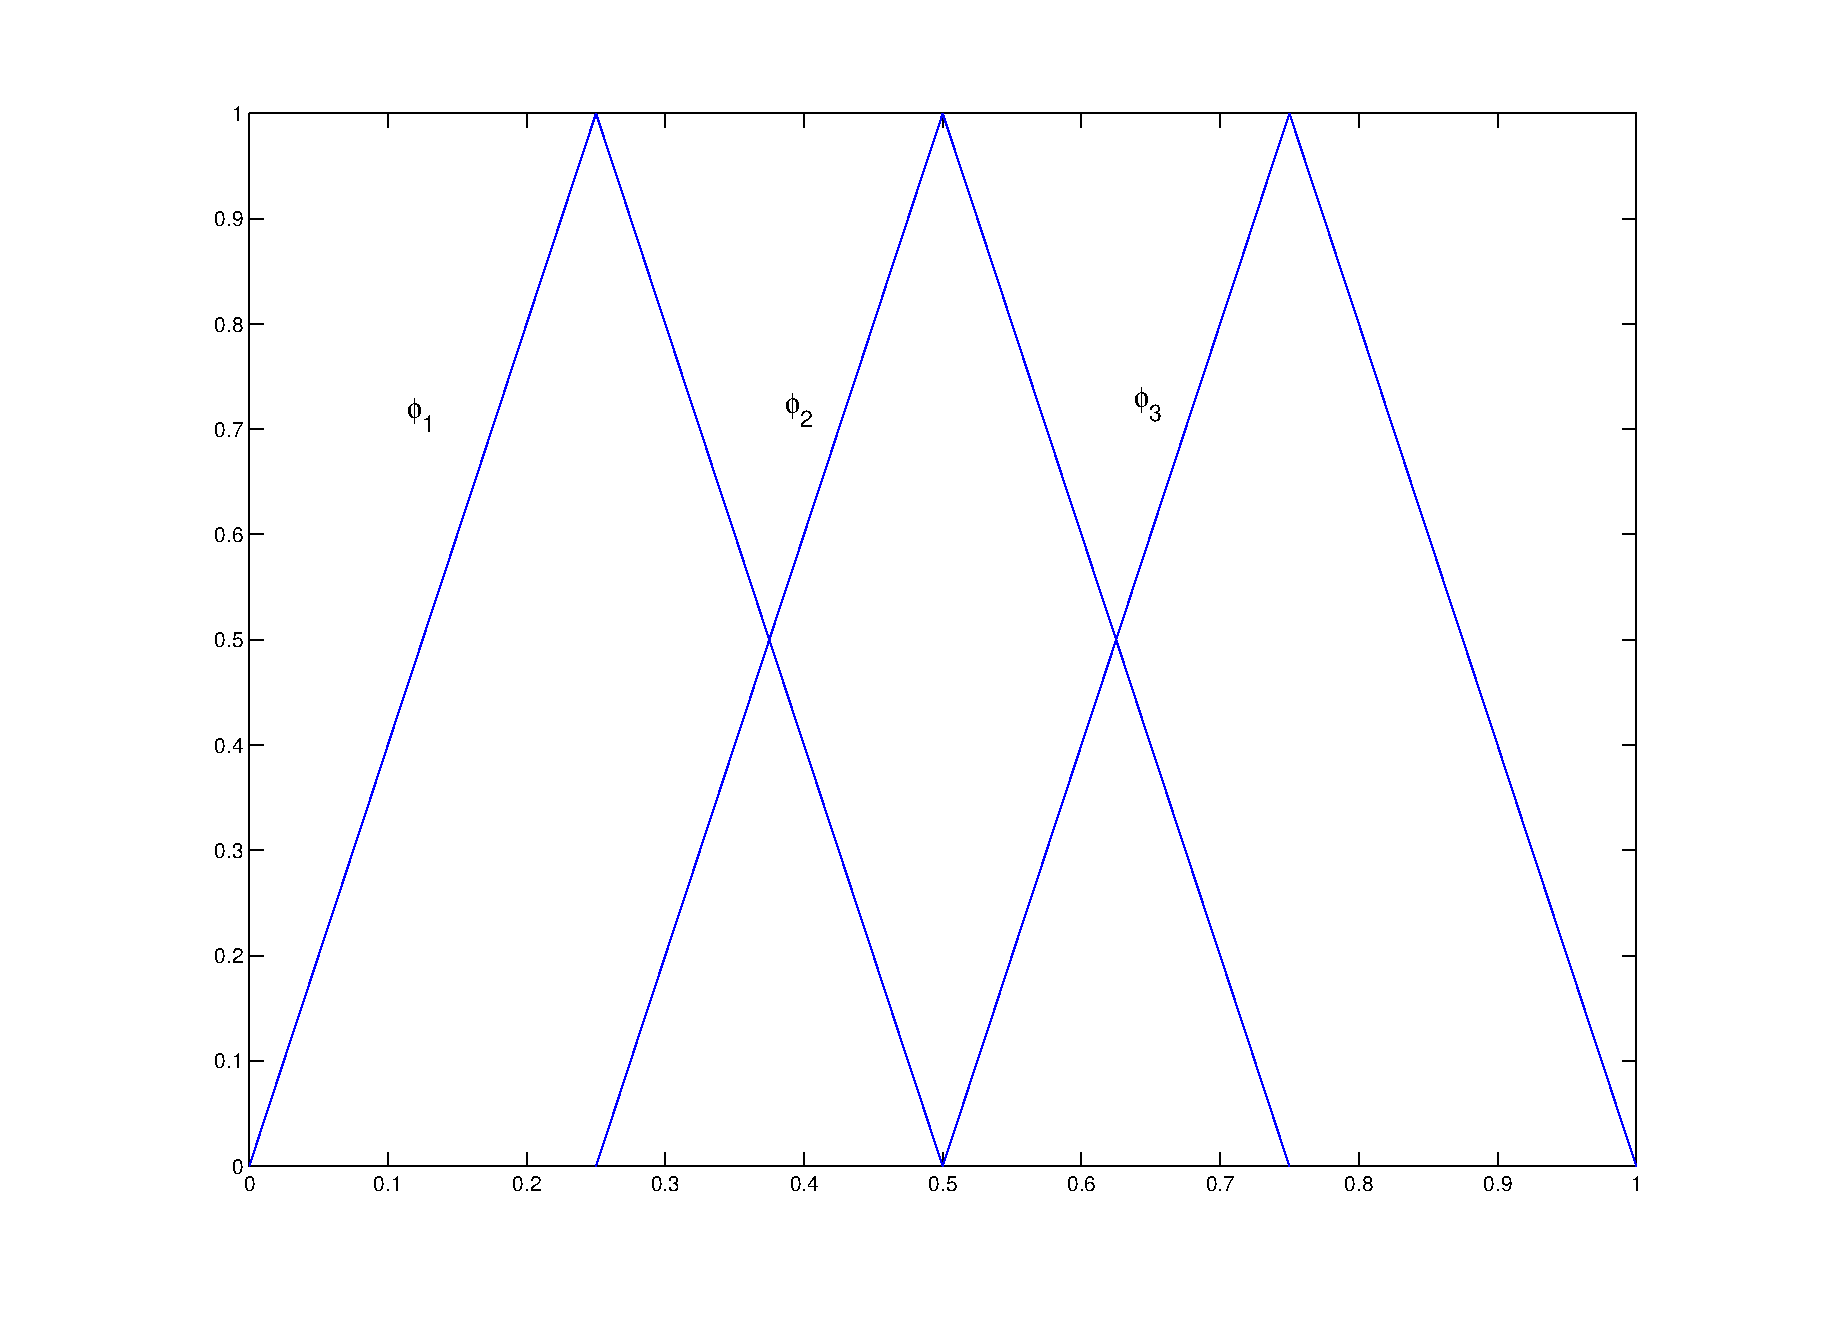
\includegraphics[width=100mm]{figure-2-1-1.eps}
\caption{hat function}
\label{fig:test}
\end{figure}

于是,$\mathbf{K}$的矩阵元$K_{ij}=\int_0^1 \frac{d \phi_1}{dx} \frac{d\phi_j}{dx}dx$为:
\begin{equation}
\mathbf{K} = \begin{bmatrix}
8 & -4 & 0 \\\\
-4 & 8 & -4 \\\\
0 & -4 & 8 
\end{bmatrix}
\end{equation}
$\mathbf{F}$的矩阵元$F_{i1} = \int_0^1 f(x) \phi_i(x)dx = \int_0^1 \phi_i(x)dx$为
\begin{equation}
\mathbf{F} = \begin{bmatrix}
\frac{1}{4}\\\\
\frac{1}{4}\\\\
\frac{1}{4}
\end{bmatrix}
\end{equation}
因此,$\mathbf{KU}=\mathbf{F}$解得:
\begin{equation}
\mathbf{U} = \begin{bmatrix}
\frac{3}{32} \\\\
\frac{1}{8} \\\\
\frac{3}{32}
\end{bmatrix}
\end{equation}

将端点处的值代入$u(x) = \sum U_i \phi_i(x) + 1$:
\begin{equation}
u(\frac{1}{4}) = \frac{35}{32}, u(\frac{1}{2}) = \frac{9}{8}, u(\frac{3}{4}) = \frac{35}{32}
\end{equation}
这与解析解在三个端点处给出的数值完全相等。
%----------------------------------------------------------------------------------------
\end{CJK*}
\end{document}
